
% http://www.math.umbc.edu/~rouben/beamer/

\documentclass[12pt]{beamer}
\usetheme{Copenhagen}

\usefonttheme{structurebold} 

\setbeamertemplate{blocks}[rounded][shadow=true] 
% itemize levels
\setbeamertemplate{itemize item}{\scriptsize\raise1.25pt\hbox{\donotcoloroutermaths$\blacksquare$}}
\setbeamertemplate{itemize subitem}{\tiny\raise1.5pt\hbox{\donotcoloroutermaths$\blacktriangleright$}}
%\setbeamertemplate{itemize subitem}{--}
\setbeamertemplate{itemize subsubitem}{\tiny\raise1.5pt\hbox{\donotcoloroutermaths$\star$}}
% enumerate levels
\setbeamertemplate{enumerate item}{\insertenumlabel.}
\setbeamertemplate{enumerate subitem}{\insertenumlabel.\insertsubenumlabel}
\setbeamertemplate{enumerate subsubitem}{\insertenumlabel.\insertsubenumlabel.\insertsubsubenumlabel}
\setbeamertemplate{enumerate mini template}{\insertenumlabel}

\setbeamertemplate{navigation symbols}{}
%\setbeamertemplate{items}[ball]
\setbeamersize{text margin left=6mm, text margin right=6mm}


%\useoutertheme{infolines}
\author{Markus Schordan and Adrian Prantl} 
\institute{FH Technikum Wien, Austria\\and\\Lawrence Livermore National Laboratory, CA, USA} 

% compatibility defs for commands used in original prosper files
\newcommand{\ptsize}[1]{\fontsize{#1}{12}\selectfont } % we ignore this command

% defs for ignoring different parts
\newcommand{\optimization}[1]{#1} % we ignore optimizations with {} (otherwise use {#1}.
\newcommand{\advancedtopic}[1]{#1} % we ignore advanced topics with {} (otherwise use {#1}.
\newcommand{\ignore}[1]{} % we ignore some slides

\usepackage{color} % load color package
%\definecolor{<color_name>}{<color model>}{<values>}

\usepackage{latexsym}
\usepackage{amssymb}   
\usepackage{epsfig}
%\usepackage{psfig}
%\usepackage{epsf}
\usepackage{graphicx}

\usepackage[utf8]{inputenc}
\usepackage[english]{babel}
\usepackage{cite}
%\usepackage[cmex10]{amsmath}   % for \split etc.
%\usepackage[usenames]{color}
\usepackage{graphicx}
%\usepackage{array}  % for tables
\usepackage{mdwtab}
\usepackage{rotating}  % for tables
\usepackage{multicol}  % for tables
\usepackage{multirow}  % for tables
\usepackage{verbatim}
\usepackage{algorithmicx}
\usepackage{algorithm2e}
%\usepackage[ruled]{algorithm}
%\usepackage{algpseudocode}
\usepackage{picture}
\usepackage[final]{pdfpages}
\usepackage{setspace}
\usepackage{alltt} % for fixed-width font sourcecode figures

% making bitmap graphics in PDF look good
% ps2pdf -dAutoFilterColorImages=false -dColorImageFilter=/FlateEncode

% transitions: Split Blinds Box Wipe Dissolve Glitter Replace (default) 
% begin{slide}[transition]{title}

% syntax for defining colors; color models can be, rgb, cmyk, gray;
% values are comma separated decimal values
% color names can be any logical name you might assign for a color

% eg:
% HEX: 006666 -> range[0,1] -> 
\definecolor{lavender}{rgb}{.0,.32,.32}
\definecolor{algomarkcolor}{rgb}{.82,.82,.42}
\definecolor{black}{rgb}{.0,.0,.0}
\definecolor{red}{rgb}{1.0,.0,.0}
\definecolor{green}{rgb}{.1,0.6,.1}
\definecolor{blue}{rgb}{.0,.0,1.0}
\definecolor{lightblue}{rgb}{.3,.3,0.8}
%
%\definecolor{gray10}{gray}{.9} % 10% gray
%
% Usage:
%
%\textcolor{lavender}{text material to appear in lavender color}
%
%or 
%
%\color{lavender} Material to appear in color .... \normalcolor
%
%or you might define environments which would start and end the
%particular color you want.
%
%Useful documentation:
%
%* grfguide.ps(.gz), which is available in any standard TeX distribution.
%
%* TUGIndia on-line tutorial which describes color table available at:
%  http://www.tug.org.in/tutorials.html 
%* proper tutorial
%  http://www.math.umbc.edu/~rouben/prosper

% how to include graphics (e.g.: 3 pics side-by-side):
%\bigskip
%\begin{center}
%    \includegraphics[height=35mm]{ns-2d-u.eps}
%    \includegraphics[height=35mm]{ns-2d-v.eps}
%    \includegraphics[height=35mm]{ns-2d-p.eps}
%\end{center}

% LOGO: \Logo{\umbclogo}
%       \Logo{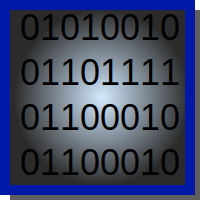
\includegraphics{logo.eps}}
%       \Logo(x,y){someobject}.

% \hyperlink{mytarget}{Click here} to go to the target slide.
% \hypertarget{mytarget}{}
% in acrobat reader: use <CTRL>+<LEFT ARROW> to return to a source-page.

% \href{run:movie.mpg}{Start Movie}

% set default font size
% \ptsize{n}, with in {8, 9, 10, 11, 12, *14*, 17}
\ptsize{12}

%\input{~/diss/thesis/formalisms}

% mehrspaltiges layout
% \begin{minipage}[t]{0.7\textwidth}
% linke seite
% \end{minipage}
% % KEINE LEERZEILE (sonst minipages untereinander)
% \begin{minipage}[t]{0.7\textwidth}
% rechte seite
% \end{minipage}

% selbstdefinierte kopf und fuSzeilen
% package fancyhdr


%\leftFOOT{Markus Schordan}
%\rightFOOT{RIGHT}
%\centerFOOT{\today}

%fake
%\newcommand{\textsc}[1]{} % 

\ptsize{10}
\def\makeactive#1{\catcode`#1 = \active\relax}
{\catcode`\^^I=\active %
 \catcode`\^^M=\active %
 \gdef\prologcode{ %
  \catcode`\^^I=\active %
  \catcode`\^^M=\active %
  \def^^I{\>} %
  \def^^M{\\[0pt]} %
 } %
}

\newenvironment{formula}
{%
\begin{displaymath}%
\begin{array}{rcl}%
}%
{%
\end{array}%
\end{displaymath}%
}%

\outcomment{
\newenvironment{example}
{%
\textbf{Example}.%
}%
{%
%
}%

\newenvironment{remark}
{%
\textbf{Remark}:%
}%
{%
%
}%

\newenvironment{proof}
{%
\textbf{Proof}:%
}%
{%
$\Box$%
}%
}

\newenvironment{PROG}                          % Prolog Umgebung
{
\begin{minipage}[t]{40ex}%
\prologcode\progfont%
\begin{quote}%
\begin{tabbing}%
\hspace{3ex}\=\hspace{3ex}\=\hspace{3ex}\=\hspace{3ex}%
\=\hspace{3ex}\=\hspace{3ex}\=\hspace{3ex}\=\hspace{3ex}\=\hspace{3ex}\=\hspace{3ex}\=\hspace{3ex}\=\hspace{3ex}\=\hspace{3ex}\kill}%
{\end{tabbing}%
\end{quote}%
\end{minipage}%
}

\newenvironment{PROGscriptsize}                          % Prolog Umgebung
{
\begin{minipage}[t]{40ex}%
\prologcode\scriptsize%
\begin{quote}%
\begin{tabbing}%
\hspace{3ex}\=\hspace{3ex}\=\hspace{3ex}\=\hspace{3ex}%
\=\hspace{3ex}\=\hspace{3ex}\=\hspace{3ex}\=\hspace{3ex}\=\hspace{3ex}\=\hspace{3ex}\=\hspace{3ex}\=\hspace{3ex}\=\hspace{3ex}\kill}%
{\end{tabbing}%
\end{quote}%
\end{minipage}%
}


%logic
\newcommand{\logand}[0]{\land}
\newcommand{\logor}[0]{\lor}
\newcommand{\lognot}[0]{\lnot}
\newcommand{\impl}[0]{\to}
\newcommand{\existsone}[0]{\exists!}
\newcommand{\notexists}[0]{\not\!\!\:\exists}

\newcommand{\ordner}[1]{ [Ordner {#1}]}

\newcommand{\pe}[1]{[{#1}]}
%sets
\newcommand{\setunion}[0]{\cup}
\newcommand{\setintersect}[0]{\cap}
\newcommand{\setdif}[0]{\backslash}
\newcommand{\tuple}[1]{({#1})}
\newcommand{\set}[1]{\{{#1}\}}
\newcommand{\pair}[2]{({#1},{#2})}
\newcommand{\tripel}[3]{({#1},{#2},{#3})}
\newcommand{\triple}[3]{({#1},{#2},{#3})}
\newcommand{\quadrupel}[4]{({#1},{#2},{#3},{#4})}

\newcommand{\cnodedef}[0]{\pair{ \set{ \pair{*}{\epsilon} } }{.} }
%\newcommand{\cnode}[0]{\diamond}
\newcommand{\cnodeset}[0]{\set{\diamond}}

%\newcommand{\bottomelement}{\tuple{\emptyset,\emptyset}}
\newcommand{\topelement}{\ensuremath{\top}}
\newcommand{\bottomelement}{\ensuremath{\perp}}
\newcommand{\dach} {\symbol{94}}
\newcommand{\deref}[1]{{#1}\dach}
\newcommand{\sname}[1]{[{#1}]}
\newcommand{\lname}[2]{[{#1},{#2}]}
\newcommand{\MSG}[0]{FSG }
\newcommand{\MSGpoint}[0]{FSG}
\newcommand{\MSGs}[0]{FSGs }
\newcommand{\MSGspoint}[0]{FSGs}
\newcommand{\MSGClass}[0]{\mathcal{\MSG}}
\newcommand{\Fcal}[0]{\mathcal{F}} % set of Functions, written as mathcal{F}.
\newcommand{\ffix}[0]{f.} % notation for fixpoint iteration
\newcommand{\mc}[1]{\multicolumn{3}{l|}{{#1}}} % multicolumn macro used in tabs for graphs
\newcommand{\kstring}[1]{\lceil {#1}]_k} % formal notation for k-truncated call strings (#1)
\newcommand{\nl}[1]{\ensuremath{\#{#1}}}

\newcommand{\edge}[1]{[{#1}]}

%\newcommand{\PP}[1]{{\em {#1}}}
\newcommand{\defeq}[0]{\stackrel{\mathrm{def}}{=}}

\newcommand{\exclude}[1]{}
\newcommand{\nsubset}{\not\subset}         %\\nsubset
%\newcommand{\textflorin}{\textit{f}}       %\\textflorin
\newcommand{\setB}{{\mathord{\mathbb B}}}  %\\setB
\newcommand{\setC}{{\mathord{\mathbb C}}}  %\\setC
\newcommand{\setN}{{\mathord{\mathbb N}}}  %\\setN
\newcommand{\setQ}{{\mathord{\mathbb Q}}}  %\\setQ
\newcommand{\setR}{{\mathord{\mathbb R}}}  %\\setR
\newcommand{\setZ}{{\mathord{\mathbb Z}}}  %\\setZ
\newcommand{\coloncolon}{\mathrel{::}}     %\\coloncolon
\newcommand{\lsem}{\mathopen{\lbrack\mkern-3mu\lbrack}}  %\\lsemantics
\newcommand{\rsem}{\mathclose{\rbrack\mkern-3mu\rbrack}} %\\rsemantics   
\newcommand{\pow}[1]{\mathcal{P}({#1})} % powerset of #1

\newcommand{\fullcirc}[0]{\bullet}
\newcommand{\heap}[0]{\mathcal{H}} % H (used for elements of the heap)
\newcommand{\nullref}[0]{\diamond} % box used as symbol for the reference value null
\newcommand{\nullnode}[0]{\ensuremath{\diamond}}
\newcommand{\recvar}[1]{\ensuremath{\bar{{#1}}}}
\newcommand{\ip}[1]{\ensuremath{\widehat{{#1}}}}% Notation for interprocedural entities 

\newcommand{\meetoperator}[0]{join operator }  % intraprocedural meet operator
\newcommand{\meet}[0]{\ensuremath{\sqcup}}  % intraprocedural meet operator
\newcommand{\imeet}[0]{\ip{\meet}}      % interprocedural meet operator
\newcommand{\bigmeet}[0]{\bigsqcup}        % big intraprocedural meet operator
\newcommand{\ibigmeet}[0]{\ip{\bigmeet}}% big interprocedural meet operator
\newcommand{\ifelse}[3]{                % if-else array for function definitions (3 parameters)
  \left\{\begin{array}{l@{\quad:\quad}l}%
      {#1} & {#2} \\%
      {#3} & \mbox{otherwise}%
    \end{array}%
  \right.}%

\newcommand{\longifelse}[4]{                % if-else array for function definitions (3 parameters)
  \left\{\begin{array}{l@{\quad:\quad}l}%
      {#1} & {#2} \\%
      {#3} & {#4} \\%
    \end{array}%
  \right.}%

\newcommand{\source}[1]{{\ttfamily #1}}
\newcommand{\progfont}[0]{\footnotesize}     % Zeichensatz 2 der Prologbeispiele
\newcommand{\mystring}[1]{"{#1}"}
\newcommand{\PP}[1]{{\progfont#1}\normalsize}
\newcommand{\ez}[0]{in }  % Das Elementzeichen
\newcommand{\anypath}[2]{{#1} *\to {#2}}
\newcommand{\nonnullpath}[2]{{#1} +\to {#2}}

\newcommand{\pathCd}[2]{{#1}{#2}}
\newcommand{\pathCa}[2]{{#1}{#2}}
\newcommand{\pathJ}[2]{{#1}{#2}}
\newcommand{\pathM}[2]{{#1}{#2}}
\newcommand{\code}[1]{{\textup\texttt {#1}}}

\newcommand{\ro}[0]{\ensuremath{\{\}}} % root in a graph

% new commands 2004

\newcommand{\emptystring}[0]{\epsilon}
\newcommand{\closurederivation}[0]{\rightarrow}
% Content: some macros for program analysis slides
% Author : Markus Schordan

% lattice terminology
\newcommand{\lle}[0]{\sqsubseteq} % lattice less or equal
\newcommand{\notlle}[0]{\not\sqsubseteq} % lattice less or equal
\newcommand{\mapto}[0]{\rightarrow}
\newcommand{\poset}[0]{{L=\pair{L}{\lle}}}
\newcommand{\transferfunction}[2]{f_{#1} : #2 \mapto #2}

% colors
\newcommand{\sourcetooptimizecol}[1]{\textcolor{red}{#1}}
\newcommand{\optimizedsourcecol}[1]{\textcolor{green}{#1}}
\newcommand{\sourcetooptimize}[1]{\framebox{\sourcetooptimizecol{#1}}}
\newcommand{\optimizedsource}[1]{\framebox{\optimizedsourcecol{#1}}}
\newcommand{\marksource}[1]{\framebox{\textcolor{blue}{#1}}}
\newcommand{\fmarksource}[1]{\framebox{\textcolor{blue}{#1}}}
\newcommand{\nonfmarksource}[1]{\textcolor{blue}{#1}}

\newcommand{\definitionname}[1]{\textcolor{colTitle}{#1}}
\newcommand{\emcolor}[1]{\textcolor{colTitle}{#1}}

\newcommand{\emcolora}[1]{\textcolor{colTitle}{#1}}
\newcommand{\emcolorb}[1]{\textcolor{green}{#1}}

% shorthands for while language
\newcommand{\tnode}[2]{[{#1}]^{#2}}
\newcommand{\ttnode}[3]{[{#1}]^{#2}_{#3}}
\newcommand{\whltest}[1]{{#1}}
\newcommand{\whlassign}[2]{{#1 := #2}}
\newcommand{\whlskip}[0]{\textup{skip}}
\newcommand{\whlif}[3]{\textup{if} ~ {#1} ~ \textup{then} ~({#2})~ \textup{else} ~({#3})}
\newcommand{\whlwhile}[2]{\textup{while}~{#1}~\textup{do}~{#2}~\textup{od}}

\newcommand{\whlvar}[1]{\textup{{#1}}}

\newcommand{\whlgtc}[2]{{\whlvar{#1} > \whlvar{#2}}}
\newcommand{\whlgtec}[2]{{\whlvar{#1} \ge \whlvar{#2}}}
\newcommand{\whlltc}[2]{{\whlvar{#1} < \whlvar{#2}}}
\newcommand{\whlltec}[2]{{\whlvar{#1} \le \whlvar{#2}}}
\newcommand{\whllteq}[2]{{\whlvar{#1} = \whlvar{#2}}}
\newcommand{\whlltneq}[2]{{\whlvar{#1} \neq \whlvar{#2}}}
\newcommand{\whlassignc}[2]{\whlassign{\whlvar{#1}}{\whlvar{#2}}}

\newcommand{\analysisin}[2]{{\textup{#1}}_{\circ}({#2})}
\newcommand{\analysisout}[2]{{\textup{#1}}_{\fullcirc}({#2})}
\newcommand{\nodelabel}[0]{\ell}
\newcommand{\ellset}[0]{\{\ell\}}
\newcommand{\extremalvalue}[0]{\iota}
\newcommand{\mappingf}[0]{f.}
\newcommand{\starsetLab}[0]{Lab$_{\star}$}

\newcommand{\whlnodeassignxal}[0]{\tnode{\whlassign{x}{a}}{\ell}}
\newcommand{\whlnodeassignxalprime}[0]{\tnode{\whlassign{x}{a}}{\ell'}}
\newcommand{\whlnodeassignxyl}[0]{\tnode{\whlassign{x}{y}}{\ell}}
\newcommand{\whlnodeassignxylj}[0]{\tnode{\whlassign{x}{y}}{\ell_j}}
\newcommand{\whlnodeassignxy}[0]{\tnode{\whlassign{x}{y}}{}}
\newcommand{\whlnodeskipl}[0]{\tnode{\whlskip}{\ell}}
\newcommand{\whlnodesequence}[0]{S_1;S_2}
\newcommand{\whlnodetestl}[0]{\tnode{b}{\ell}}
\newcommand{\whlnodeifl}[0]{\whlif{\whlnodetestl}{S_1}{S_2}}
\newcommand{\whlnodewhilel}[0]{\whlwhile{\whlnodetestl}{S}}

\newcommand{\whlnodecallcr}[0]{\ttnode{\textup{call}~p(a,z)}{\ell_c}{\ell_r}}
\newcommand{\whlnodeprocedurexn}[0]{\textup{proc}~p(\textup{val}~x;~\textup{res}~y)~\textup{is}^{\ell_n}~S~\textup{end}^{\ell_x}}


\newcommand{\auxlabels}[1]{\textup{labels}(#1)}
\newcommand{\auxinit}[1]{\textup{init}(#1)}
\newcommand{\auxfinal}[1]{\textup{final}(#1)}
\newcommand{\auxflow}[1]{\textup{flow}(#1)}
\newcommand{\auxflowr}[1]{\textup{flow}^{R}(#1)}
\newcommand{\auxblocks}[1]{\textup{blocks}(#1)}
\newcommand{\auxS}[0]{S_\star}

\newcommand{\auxkill}[2]{\textup{kill}_{\textup{#1}}(#2)}
\newcommand{\auxgen}[2]{\textup{gen}_{\textup{#1}}(#2)}
\newcommand{\auxskill}[1]{\ensuremath{\textup{kill}_{#1}}} % short kill
\newcommand{\auxsgen}[1]{\textup{gen}_{#1}} % short gen

\newcommand{\varstar}[0]{\textup{Var}_\star}
\newcommand{\Varstar}[0]{\textup{Var}_\star}
\newcommand{\SAALoc}[0]{\textup{ALoc}}
\newcommand{\SASel}[0]{\textup{Sel}}
\newcommand{\SAAState}[0]{\textup{AState}}
\newcommand{\SAAHeap}[0]{\textup{AHeap}}
\newcommand{\SAIsShared}[0]{\textup{IsShared}}
\newcommand{\SAS}[0]{\textup{S}}
\newcommand{\SAH}[0]{\textup{H}}
\newcommand{\SAis}[0]{\textup{is}}
\newcommand{\SASG}[0]{\textup{SG}}
\newcommand{\SAsgtriple}[0]{(\SAS,\SAH,\SAis)}
\newcommand{\SAtfname}[0]{f_\ell^{\textup{SA}}}
\newcommand{\SAtfmapping}[0]{\SAtfname : \pow{\SASG} \mapto \pow{\SASG}}
\newcommand{\SAsubtfname}[0]{\phi_\ell^{\textup{SA}}}
\newcommand{\SAsubtf}[1]{\SAsubtfname(#1)}
\newcommand{\SAsubtfmapping}[0]{\SAsubtfname : \SASG \mapto \pow{\SASG}}
\newcommand{\SAPExp}[0]{\textup{PExp}}

\newcommand{\equationininit}[3]{ % (analysisname,label,initvalue)
\analysisin{#1}{#2}&=&{#3}\\
}
\newcommand{\equationinidentity}[3]{ % (analysisname,labelLHS,labelRHS)
\analysisin{#1}{#2}&=&\analysisout{#1}{#3}\\
}
\newcommand{\equationoutidentity}[2]{ % (analysisname,label)
\analysisout{#1}{#2}&=&\analysisin{#1}{#2}\\
}
\newcommand{\equationoutkillgen}[4]{ % (analysisname,label,killset,genset)
\analysisout{#1}{#2}&=&\analysisin{#1}{#2}~\setdif~{#3}~\setunion~{#4}\\
}
\newcommand{\equationincombination}[5]{ % (analysisname,labelLHS,labelRHS1,combinationop,labelRHS2)
\analysisin{#1}{#2}&=&\analysisout{#1}{#3}~{#4}~\analysisout{#1}{#5}\\
}
\newcommand{\algokillgen}[1]{
(\analysisin{#1}{\ell}\setdif \textup{kill}_\textup{#1}(B^\ell))~\setunion~\textup{gen}_\textup{#1}(B^\ell)
}

\newcommand{\exampleprogramfactorial}[0]{
Example:% {\em Factorial}
\\
$\tnode{\whlassignc{y}{x}}{1};
\tnode{\whlassignc{z}{1}}{2};
\whlwhile{\tnode{\whlgtc{y}{1}}{3}}
  {\tnode{\whlassignc{z}{z $\ast$ y}}{4};
   \tnode{\whlassignc{y}{y $-$ 1}}{5}
  };
\tnode{\whlassignc{y}{0}}{6}
$
}

\newcommand{\elementaryblockgraph}[2]{ %(analysisname,elementaryblock) 
\begin{picture}(100,60)
\put(30,43){\textup{{#1}}$_\circ$($\ell$)}
\put(2,25){\framebox{${#2}$}}
\put(30,7){\textup{{#1}}$_\fullcirc$($\ell$)}

\put(24,58){\vector(0,-1){21}}
\put(24,19){\vector(0,-1){21}}
\end{picture}
}

\newcommand{\elementaryblockgraphbackward}[2]{ %(analysisname,elementaryblock) 
\begin{picture}(100,60)
\put(30,43){\textup{{#1}}$_\circ$($\ell$)}
\put(2,25){\framebox{${#2}$}}
\put(30,7){\textup{{#1}}$_\fullcirc$($\ell$)}

\put(24,37){\vector(0,1){21}}
\put(24,-2){\vector(0,1){21}}
\end{picture}
}

\newcommand{\allelementaryblocksgraph}[1]{
\begin{tabular}{r|r|r}
\elementaryblockgraph{#1}{\whlnodeassignxal}
&
\elementaryblockgraph{#1}{~~~~\whlnodetestl~~~~}
&
\elementaryblockgraph{#1}{~\whlnodeskipl~}\\\hline
\end{tabular}
}

\newcommand{\allelementaryblocksgraphbackward}[1]{
\begin{tabular}{r|r|r}
\elementaryblockgraphbackward{#1}{\whlnodeassignxal}
&
\elementaryblockgraphbackward{#1}{~~~~\whlnodetestl~~~~}
&
\elementaryblockgraphbackward{#1}{~\whlnodeskipl~}\\\hline
\end{tabular}
}

\newcommand{\basicideagraph}[2]{
\bigskip
\begin{center}
\begin{tabular}{l|r}
\elementaryblockgraph{#1}{\whlnodeassignxal}
&
\begin{picture}(100,60)
\put(30,50){\framebox{$\tnode{...}{\ell_1}$}}
\put(10,35){\textup{{#1}}$_\fullcirc$($\ell_1$)}
\put(90,50){\framebox{$\tnode{...}{\ell_2}$}}
\put(105,35){\textup{{#1}}$_\fullcirc$($\ell_2$)}

\put(91,9){\textup{{#1}}$_\circ$($\ell$)}
\put(62,0){\framebox{$\tnode{...}{\ell}$}}

\put(46,44){\vector(2,-3){21}}
\put(102,44){\vector(-2,-3){21}}
\put(70,21){{#2}} % combination operator
\end{picture}
\end{tabular}
\end{center}
\bigskip
}

\newcommand{\basicideagraphbackward}[2]{
\bigskip
\begin{center}
\begin{tabular}{l|r}
\elementaryblockgraphbackward{#1}{\whlnodeassignxal}
&
\begin{picture}(100,60)
\put(30,2){\framebox{$\tnode{...}{\ell_1}$}}
\put(10,18){$\analysisin{#1}{\ell_1}$}
\put(90,2){\framebox{$\tnode{...}{\ell_2}$}}
\put(108,18){$\analysisin{#1}{\ell_2}$}

\put(92,41){$\analysisout{#1}{\ell}$}
\put(62,49){\framebox{$\tnode{...}{\ell}$}}

\put(102,14){\vector(-2,3){20}}
\put(46,14){\vector(2,3){20}}
\put(70,31){{#2}} % combination operator
\end{picture}
\end{tabular}
\end{center}
\bigskip
}

\newcommand{\bitvectorrhscombination}[4]{ %(analysisName,InitialValue,CombOp,extremalValueSet)
\longifelse{{#2}}{\textup{if}~\ell={#4}}{{#3} \{\analysisout{#1}{\ell'}|\tuple{\ell',\ell}\in \auxflow{\auxS}\}}{\textup{otherwise}}
}

\newcommand{\bitvectorrhscombinationbackward}[4]{ %(analysisName,InitialValue,CombOp,extremalValueSet)
\longifelse{{#2}}{\textup{if}~\ell={#4}}{{#3} \{\analysisin{#1}{\ell'}|\tuple{\ell',\ell}\in \auxflowr{\auxS}\}}{\textup{otherwise}}
}

\newcommand{\bitvectorrhskillgen}[2]{ %(analysisname,analysisrhs{analysisname})
({#2}\setdif \textup{kill}_\textup{#1}(B^\ell))~\setunion~\textup{gen}_\textup{#1}(B^\ell) ~~~~\textup{where}~B^\ell\in\auxblocks{S_\star}
}

\newcommand{\bitvectoranalysisin}[3]{ %(analysisname,InitialValue,CombOp)
\analysisin{#1}{\ell}&=&\bitvectorrhscombination{#1}{#2}{#3}{\auxinit{\auxS}}
}

\newcommand{\bitvectoranalysisout}[1]{ %(analysisname)
\analysisout{#1}{\ell}&=&\bitvectorrhskillgen{#1}{\analysisin{#1}{\ell}}
}

\newcommand{\bitvectoranalysisinbackward}[1]{ %(analysisname)
\analysisin{#1}{\ell}&=&\bitvectorrhskillgen{#1}{\analysisout{#1}{\ell}}
} 

\newcommand{\bitvectoranalysisoutbackward}[3]{ %(analysisname,InitialValue,CombOp)
\analysisout{#1}{\ell}&=&\bitvectorrhscombinationbackward{#1}{#2}{#3}{\auxfinal{\auxS}}
}

\newcommand{\bitvectoranalysis}[3]{%(Name,InitialValue,CombinationOperator}
\begin{formula}
\bitvectoranalysisin{#1}{#2}{#3}\\
\bitvectoranalysisout{#1}
\end{formula} 
}

\newcommand{\bitvectoranalysisbackward}[3]{%(Name,InitialValue,CombinationOperator}
\begin{formula}
\bitvectoranalysisinbackward{#1}\\
\bitvectoranalysisoutbackward{#1}{#2}{#3}
\end{formula} 
}

\newcommand{\elementaryblocksanalysis}[7]{ % (AnalysisName,kill-assign,kill-skip,kill-b,gen-assign,gen-skip,gen-b)
\allelementaryblocksgraph{#1}
\begin{formula}
\textup{kill}_{\textup{#1}}(\tnode{\whlassign{x}{a}}{\ell})&=&{#2}\}\\
\textup{kill}_{\textup{#1}}(\tnode{\whlskip}{\ell})&=&{#3}\\
\textup{kill}_{\textup{#1}}(\tnode{\whltest{b}}{\ell})&=&{#4}\\
\textup{gen}_{\textup{#1}}(\tnode{\whlassign{x}{a}}{\ell})&=&{#5}\\
\textup{gen}_{\textup{#1}}(\tnode{\whlskip}{\ell})&=&{#6}\\
\textup{gen}_{\textup{#1}}(\tnode{\whltest{b}}{\ell})&=&{#7}\\
\end{formula}

\begin{formula}
\bitvectoranalysisout{#1}
\end{formula}
}

\newcommand{\elementaryblocksanalysisbackward}[7]{ % (AnalysisName,kill-assign,kill-skip,kill-b,gen-assign,gen-skip,gen-b)
\allelementaryblocksgraphbackward{#1}
\begin{formula}
\textup{kill}_{\textup{#1}}(\tnode{\whlassign{x}{a}}{\ell})&=&{#2}\\
\textup{kill}_{\textup{#1}}(\tnode{\whlskip}{\ell})&=&{#3}\\
\textup{kill}_{\textup{#1}}(\tnode{\whltest{b}}{\ell})&=&{#4}\\
\textup{gen}_{\textup{#1}}(\tnode{\whlassign{x}{a}}{\ell})&=&{#5}\\
\textup{gen}_{\textup{#1}}(\tnode{\whlskip}{\ell})&=&{#6}\\
\textup{gen}_{\textup{#1}}(\tnode{\whltest{b}}{\ell})&=&{#7}\\
\end{formula}

\begin{formula}
\bitvectoranalysisinbackward{#1}
\end{formula}
}

\newcommand{\basicanalysisinformation}[4]{ % (AnalysisName,AinText,AoutText,killText,genText)
Analysis information: $\analysisin{#1}{\nodelabel}$,$\analysisout{#1}{\nodelabel}$ : $\textup{Lab}_\star \rightarrow \pow{#4}$

\begin{itemize}
\item $\analysisin{#1}{\nodelabel}$: {#2} {#3} \definitionname{entry} of block $\nodelabel$.
\item $\analysisout{#1}{\nodelabel}$: {#2} {#3} \definitionname{exit} of block $\nodelabel$.
\end{itemize}

}

\newcommand{\basicanalysisproperties}[3]{ %(Direction, MayMust, Combination Operator)
Analysis properties:
\begin{itemize}
\item Direction: {#1} 
\item #2 analysis with combination operator #3
\end{itemize}
}

\outcomment{
\newcommand{\forwardalgorithm}[5]{ % (analysisname,init,topelem,fixpointtestop,combinationop)
\begin{sourcecode}
W:=nil;\\
foreach $\pair{\ell}{\ell'} \in \auxflow{S_\star}~\textup{do}$ W := cons($\pair{\ell}{\ell'}$,W); od;\\
foreach $\ell \in \auxlabels{S_\star}~\textup{do}$\\
\>if $\ell=\auxinit{S_\star}$ then \\
\>\>$\analysisin{#1}{\ell} := $\colorbox{algomarkcolor}{$#2$}\\
\>else\\
\>\> $\analysisin{#1}{\ell}:= $\colorbox{algomarkcolor}{$#3$}\\
\>fi\\
od\\
while $W \neq nil$ do\\
\> $\pair{\ell}{\ell'}$ := head(W);\\
\> W := tail(W);\\
\> if $\algokillgen{#1}$ \colorbox{algomarkcolor}{$#4$} $\analysisin{#1}{\ell'}$ then\\
\>\> $\analysisin{#1}{\ell'}$ := $\analysisin{#1}{\ell'}$ \colorbox{algomarkcolor}{$#5$} $\algokillgen{#1}$;\\
\>\> foreach $\ell''$ with $\pair{\ell'}{\ell''}$ in $\auxflow{S_\star}$ do\\
\>\>\> W := cons($\pair{\ell'}{\ell''}$,W);\\
\>\> od\\
\> fi\\
od\\
\end{sourcecode}
}
}

\newcommand{\forwardalgorithm}[5]{ % (analysisname,init,topelem,fixpointtestop,combinationop)
\genericworklistalgorithm{#1}{#2}{#3}{#4}{#5}{\auxflow{S_\star}}{\auxinit{S_\star}}
{\algokillgen{#1}}
{\auxlabels{S_\star}}
}

\newcommand{\genericworklistalgorithm}[9]{ % 
% (
% 1 analysisname,
% 2 iota,
% 3 topelem,
% 4 fixpointtestop,
% 5 combinationop,
% 6 flow,
% 7 initlabelset,
% 8 transferfunctioncall
% 9 all programlabels set
% )
% localy redefine macro \analysisin[2] to get a different analysis results notation
\begin{sourcecode}
W:=nil;\\
foreach $\pair{\ell}{\ell'} \in {#6}~\textup{do}$ W := cons($\pair{\ell}{\ell'}$,W); od;\\
foreach $\ell \in #9~\textup{do}$\\
\>if $\ell \in {#7}$ then \\
\>\>$\analysisin{#1}{\ell} := $\colorbox{algomarkcolor}{$#2$}\\
\>else\\
\>\> $\analysisin{#1}{\ell}:= $\colorbox{algomarkcolor}{$#3$}\\
\>fi\\
od\\
while $W \neq nil$ do\\
\> $\pair{\ell}{\ell'}$ := head(W);\\
\> W := tail(W);\\
\> if ${#8}$ \colorbox{algomarkcolor}{$#4$} $\analysisin{#1}{\ell'}$ then\\
\>\> $\analysisin{#1}{\ell'}$ := $\analysisin{#1}{\ell'}$ \colorbox{algomarkcolor}{$#5$} ${#8}$;\\
\>\> foreach $\ell''$ with $\pair{\ell'}{\ell''}$ in ${#6}$ do\\
\>\>\> W := cons($\pair{\ell'}{\ell''}$,W);\\
\>\> od\\
\> fi\\
od\\
\end{sourcecode}
}

\newcommand{\RDextremalvalue}[0]{\{\pair{x}{?} \mid x\in FV(S_\star)\}}
\newcommand{\RDcombop}[0]{\setunion}
\newcommand{\AEextremalvalue}[0]{\emptyset}
\newcommand{\AEcombop}[0]{\setintersect}

\newcommand{\LVextremalvalue}[0]{\emptyset} %NNHSlides:{\textup{Var}_{\star}}
\newcommand{\LVcombop}[0]{\setunion}
\newcommand{\VBEextremalvalue}[0]{\emptyset}
\newcommand{\VBEcombop}[0]{\setintersect}

\newcommand{\SAextremalvalue}[0]{\iota}
\newcommand{\SAcombop}[0]{\setunion}

\newcommand{\cube}[8]{
\begin{picture}(140,80)
\put(50, 5){\line( 0,1){25}}

\put(50, 5){\line(-2, 1){47}}
\put(50, 5){\line( 2, 1){47}}

\put(50,30){\line(-2, 1){47}}
\put(50,30){\line( 2, 1){47}}

\put(50,55){\line(-2,-1){47}}
\put(50,55){\line( 2,-1){47}}

\put(50,80){\line(-2,-1){47}}
\put(50,80){\line( 2,-1){47}}

\put(50,55){\line( 0,1){25}}

\put( 2,30){\line( 0,1){25}}
\put(98,30){\line( 0,1){25}}

% points; texts with offset y-10
%   middle
\put(50,6 ){\circle*{4}} \put(60,2){$#1$}
\put(50,31){\circle*{4}} \put(60,27){$#3$}
\put(50,55){\circle*{4}} \put(60,53){$#6$}
\put(50,80){\circle*{4}} \put(60,78){$#8$}
%   left
\put(2 ,30){\circle*{4}} \put(12,28){$#2$}
\put(2 ,55){\circle*{4}} \put(12,53){$#5$}
%   right
\put(97,30){\circle*{4}} \put(107,28){$#4$}
\put(97,55){\circle*{4}} \put(107,53){$#7$}

\end{picture}
}

\newcommand{\generalformulationinterproc}{
% 6 statements (per statement: , per arrow between statements: )
{
\ptsize{8}
\begin{picture}(220,150)
\put(196,130){proc $p$(val $x$; res $y$)}
\put(196,100){\framebox{$\tnode{\textup{is}}{\ell_n}$}}
\put(209,95){\vector(0,-1){75}}
\put(196,10){\framebox{$\tnode{\textup{end}}{\ell_x}$}}

\put(100,72){\vector(3,1){96}}
\put(196,15){\vector(-3,1){96}}
\put(40,58){$\whlnodecallcr$}
\put(50,62){\oval(100,60)}

\put(35,140){\vector(0,-1){48}}
\put(35,87){\vector(0,-1){53}} % going through line/edge
\put(35,32){\vector(0,-1){48}}

\put(42,72){\vector(1,0){56}}
\put(45,82){\oval(20,20)[bl]}
\put(98,47){\line(-1,0){54}}
\put(45,37){\oval(20,20)[tl]}

\put(22,100){X}
\put(22,56){X}
\put(40,20){$f_{\ell_c,\ell_r}(X,Y)$}

\put(120,95){$f_{\ell_c}(X)$}
\put(120,25){$Y$}

\put(215,60){body}

\end{picture}
}
}


\title{CodeThorn 1.2}
\subtitle{Conceptual Overview\\(in preparation)}
%\author{{\large Markus Schordan}}
%\institution{Institut ....}
%\slideCaption{\textit{Markus Schordan \hspace{4.5cm} \today} \hspace{4.5cm}}
%\hypersetup{colorlinks=true,linkcolor=red}

\begin{document}
\maketitle

% beamer options [...]: fragile,shrink=N (N in percent to shrink slide), squeeze (reduce gaps)
%\logo{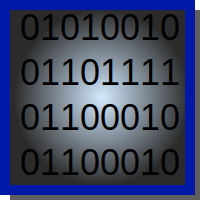
\includegraphics[height=0.5cm]{logo}}
\ignore{
\begin{frame}{Questions of Interest}
\begin{itemize}
\item How can we specify and verify the input/output behavior of a program?
\item What is relevant structural information about a program?
\item What are good methods for filtering or querying the computed program information?
\end{itemize}
\end{frame}

\begin{frame}{Scope of Program Information}
\begin{itemize}
\item Intra-procedural information
\item Inter-procedural information
\item Program slices
\item Patterns
\begin{itemize}
\item design pattern
\item data access pattern
\item Communication pattern
\end{itemize}
\item Program representation
\item Program states and transitions
\item Input/Output behavior (linear time logic formulae)
\end{itemize}

\end{frame}

\begin{frame}{Program Structures as Graphs}
\begin{itemize}
\item Abstract syntax tree (AST)
\item Inheritance hierarchy (tree/DAG)
\item Flow graphs
\begin{itemize}
\item Control flow graph
\item Control dependence graph
\item Data flow graph
\item Data dependence graph
\end{itemize}
\item Call graph
\item Collaboration graph
\item Coupling graph
\item Program dependence graph
\item State transition graph
\end{itemize}
\end{frame}
} % end of ignore

\begin{frame}{Analysis Overview}

\begin{block}{Five Phases}
\begin{enumerate}
\item Syntactic and semantic analysis of the input program (ROSE).
\item Control flow analysis.
\item General Data Flow analysis.
\begin{itemize}
\item During this analysis the state transition graph is computed.
\end{itemize}
\item LTL-Checking. 
\begin{itemize}
\item Input to the LTL-Checking phase is the state transition graph and the LTL-formulae.
\end{itemize}
\item Reporting of analysis results. 
\begin{itemize}
\item Assert reachability is computed based on the transition graph.
\item Results for LTL-formulae are computed solely by the LTL-checker.
\end{itemize}
\end{enumerate}

\end{block}
\end{frame}

\begin{frame}[fragile]
\frametitle{Folded State Transition Graph}

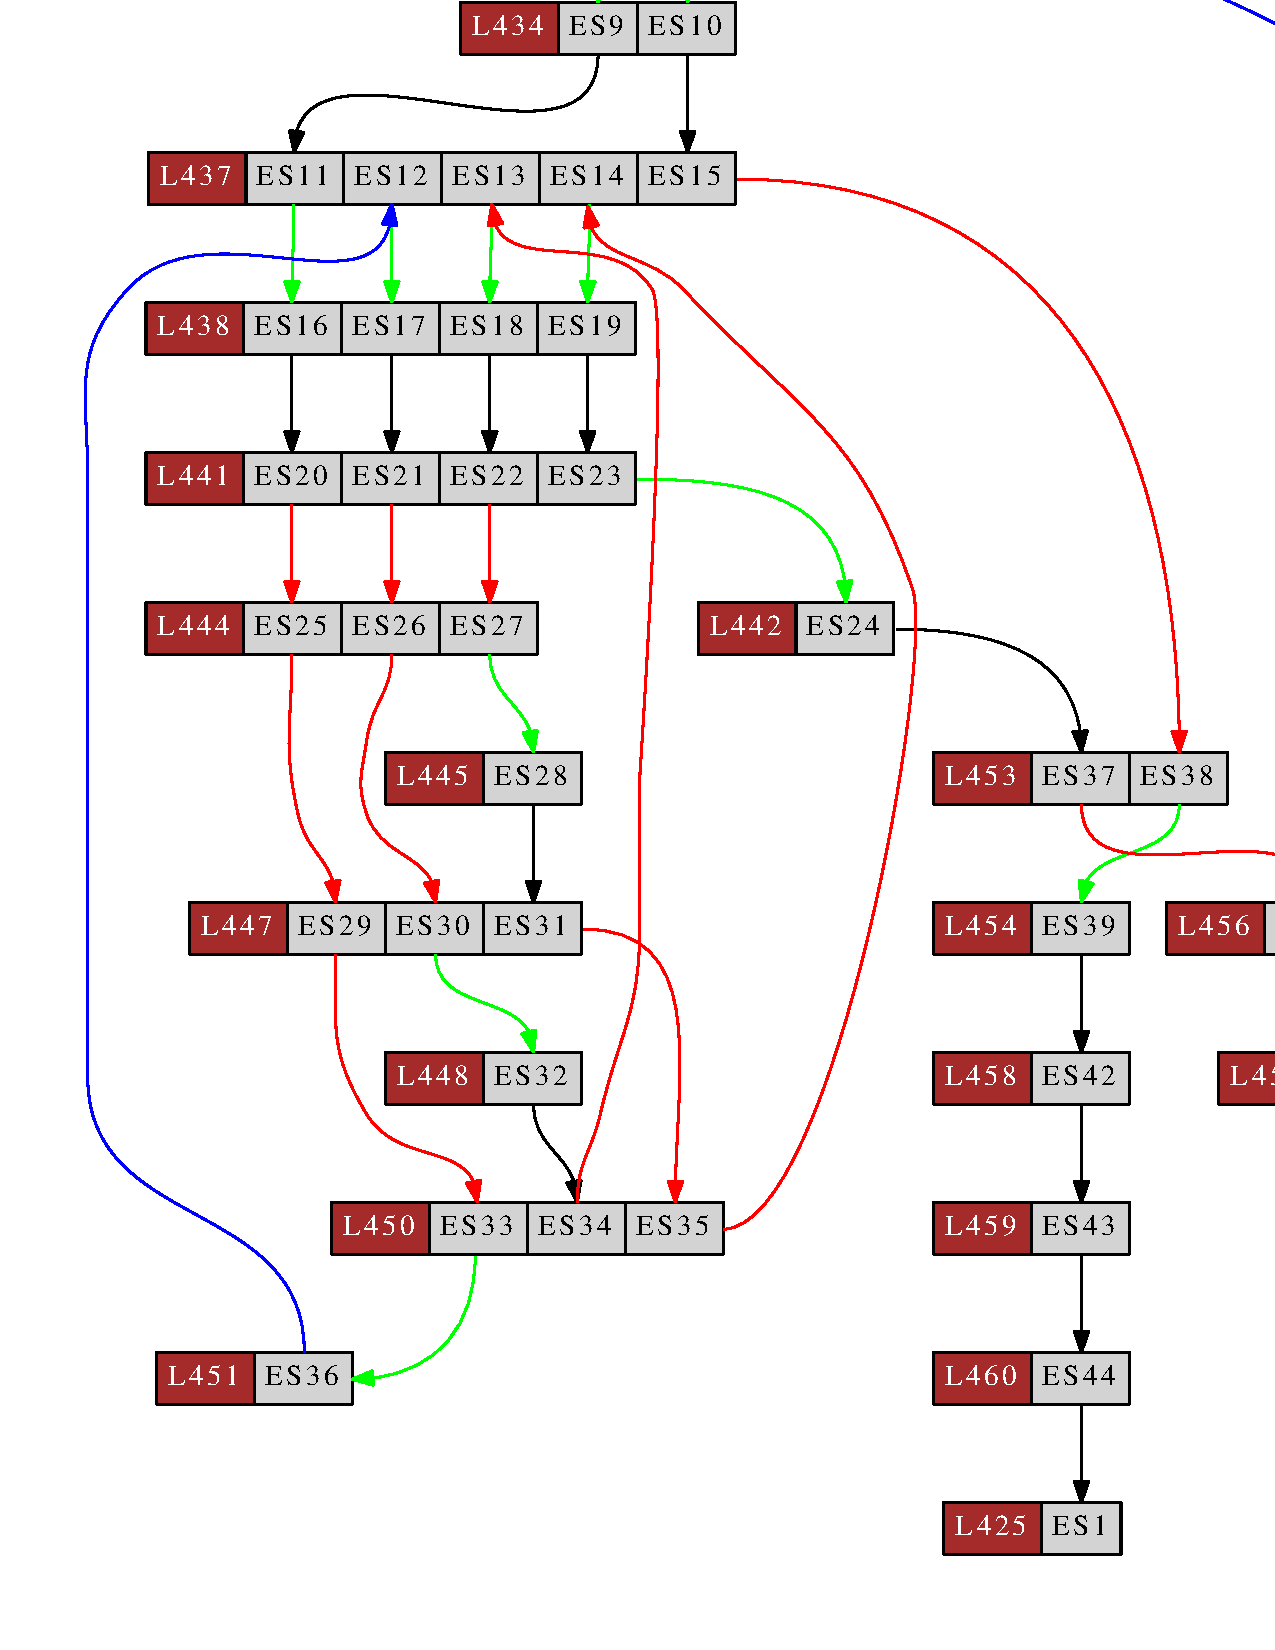
\includegraphics[width=0.4\columnwidth]{../manual/gfx/basictest10f_transitiongraph2}
% container size: 1000
% iterations: 100
% time in milliseconds?

\vspace{-0.3cm}
{
\scriptsize
\begin{block}{Edges}
\begin{itemize}
\item Cycles: Blue edges: backward edges (for identical system states)
\item Green/red edges: true/false edges
\item Black: forward edges
\end{itemize}
\end{block}
}

\end{frame}

\begin{frame}[fragile]
\frametitle{General Program Analysis Algorithm}
{
\scriptsize
\begin{algorithm}[H]
\SetLine
\KwIn{ICFG}
\KwOut{Transition Graph G}

%\ForEach{Task $i$}{
%\ForEach{Processor $j$}{
%Calculate EW($i$,$j$)\;
%\If{EW($i$,$j$) $\le$ EW($a$,$b$)}{
%$a$ = $i$\;
%$b$ = $j$\;
%}
%}
%}

$S_1$=init(ICFG) \Comment{the initial state computed from global scope and initial ICFG node}
$W$=$\{(S_0,a_0,S_1)\}$; \Comment{with $S_0$ being the empty state, $S_1$ the initial state,}\\
\Comment{and $a_0$ the initial transition annotation}\\
$T_G$=$\emptyset$; \Comment{the set of computed transitions}\\
\While{W $\neq$ $\emptyset$}{
  ($S$,$a$,$S'$):=$head(W)$; \Comment{$a$ corresponds to the respective ICFG edge type}\\
  $W$:=tail($W$)\;
  $T$:=transfer(($S$,$a$,$S'$))\;
  \ForEach{$t$ $\in$  $T$}{
    \uIf{$t$ $\notin$ $T_G$}{
        $W$:=$W$ $\cup$ $\{t\}$\;
    }\Else{
         $G$:=$G$ $\cup$ $\{t\}$\;
    }
  } 
}
%\caption{Algorithm for computing the state transition graph}
\label{alg:general}
\end{algorithm}
}
\end{frame}

\begin{frame}{Properties of the Analysis}
\begin{itemize}
\item The C files of the RERS-problems are used unmodified.
\item The data-flow analysis does not require information about possible input values of a
  given program. 
\begin{itemize}
\item All information, which is then represented in the
  transition graph, is extracted from the program code. 

\item The set of all
  possible input values is represented by the extracted constraint
  sets (as they are back-propagated from called functions to the
  main-function). 
\item The possible output values are represented in the
  property state as computed for the output operation (printf).
\end{itemize}
\item The LTL-Checker only depends on the extracted state transition graph.
\item We do not provide manually any information to the analyzer.
\end{itemize}

\end{frame}

\begin{frame}{System State (Nodes in the TG)}

\begin{block}{System State}
A system state consists of
\begin{itemize}
\item a label (lab), 
\item a property state (pstate),
\item a constraint set (cset),
\item and an IO property (io).
\end{itemize}

PState = Var $\rightarrow$ Val where Val is a lifted integer set.\\
SState = Lab $\times$ PState $\times$ ConstraintSet $\times$ IO\\
\end{block}

\begin{block}{Representation in Memory with unique Id}
\begin{itemize}
\item Label: num
\item PState: VarId $\rightarrow$ Val
\item SState: Label $\times$ PStateId $\times$ ConstraintSetId $\times$ IOId
\end{itemize}
\end{block}


\end{frame}

\begin{frame}{Normalized Minimal Constraint Sets}
\begin{block}{Minimal Constraint Set}
A minimal constraint set (MCS) is a representation of
information about the variables and values with a minimal number of operators.
\end{block}

\begin{block}{Normalized}
For any combination of operators and operands there exists exactly one representation as constraint set.
\end{block}

\begin{block}{Importance of Properties}
\begin{itemize}
\item Determining equality of system states
\item Reducing memory consumption
\end{itemize}
\end{block}

\end{frame}

\begin{frame}{Normalized Minimal Constraint Set Rules}
\begin{itemize}
\item If an equality $x=c$ exists, then no inequality $x\neq c$ on x can exist.
\item There can exist at most on equality $x=c$ on the same variable.
\item Multiple inequalities $x \neq c_i$ can exist for a given variable.
\item If there exists at least one inequality $x\neq c_i$ then no equality $x=c_j$ can exist ($i\neq j$).
\item If there exist equalities $x_0=x_1$,$x_0=x_2$$...$ then one of the variables is the {\em dedicated variable} $x_0$.
\item For any set of variable-equalities all inequalities are associated with the dedicated variable.
\item If the dedicated variable is removed from the set then all constraints are remapped.
\end{itemize}
\end{frame}

\begin{frame}{Normalized Minimal Constraint Set}

\begin{block}{Example}

\begin{itemize}
\item $C_1=\{x\neq 1, x\neq 2, x=y, x=z\}_x$ 
\begin{itemize}
\item Remove $x$ $\Rightarrow$ : $\{y\neq 1, y\neq 2, y=z\}_y$
\item Remove $z$ $\Rightarrow$ : $\{y\neq 1, y\neq \}_{\circ}$
\item add $y=z$ $\Rightarrow$ : $\{y\neq 1, y\neq, y=z\}_y$
\item add $x=z$ $\Rightarrow$ : $\{x\neq 1, x\neq 2, x=y, x=z\}_x=C_1$
\end{itemize}
\end{itemize}

\end{block}

\end{frame}

\begin{frame}{Representation in Memory}

\begin{block}{Maintainer}
Assigns memory and id to each
\begin{itemize}
\item Property State
\item Constraint Set
\item System State (includes PState and CSet)
\end{itemize}

Label and IO are maintained separately.
\end{block}

\begin{block}{Transition}
A transition is represented as $(S,a,S')$ where $S$ and $S'$ are system states and $a$
is an annotation representing the edge-type of the corresponding ICFG edge.
\end{block}

\end{frame}

\begin{frame}{Results}
\begin{center}
\vspace{-0.2cm}
\begin{tabular}{|c|l|l|}\hline
P & ASSERT & LTL \\\hline\hline
1 & W:yes+no+unknown      & W (+B:no)\\\hline
2 & W:yes+no+unknown     & W (+B:no)\\\hline
3 & W:yes+no+unknown     & W (+B:no)\\\hline
4 & W:yes+no+unknown     & W (+B:no)\\\hline
5 & W:yes+no+unknown     & (W) (+B:no)\\\hline
6 & W:yes+no+unknown     & W (+B:no) \\\hline
7 & W*:yes     & B:no    \\\hline
8 & W*:yes     & B:no    \\\hline
9 & W*:yes     & B:no    \\\hline
10 & W*:yes     & B:no    \\\hline
11 & W*:yes     & B:no    \\\hline
12 & W*:yes     & B:no    \\\hline
13 & W*:yes     & B:no    \\\hline
14 & W*:yes     & B:no    \\\hline
\end{tabular}
\end{center}
\end{frame}

\begin{frame}{Statistics}
\begin{center}
\begin{tabular}{|c|r|r|r|r|}\hline
Problem & \#PStates &\#SStates &\#Trans &\#CSets \\\hline\hline
1 &1134 & 20946 & 21194 & 32 \\\hline
2 &736 & 15261 & 15443 & 33 \\\hline
3 &1012 & 41207 & 41466 & 32 \\\hline
4 &10260 & 1125843 & 1127863 & 68 \\\hline
5 &21803 & 3466688 & 3469608 & 95 \\\hline
6 &14506 & 1665785 & 1668109 & 81 \\\hline
\end{tabular}
\end{center}
\end{frame}

\begin{frame}{Measurements (Run-Time)}
\begin{center}
\begin{tabular}{|c|r|c|}\hline
Problem& Analysis Time & Threads\\\hline\hline
1& 4.1044 secs & 12\\\hline
2& 3.1855 secs& 12\\\hline
3& 10.3215 secs& 12\\\hline
4& 3.3922 mins& 12\\\hline
5& 8.4049 mins& 12\\\hline
6& 5.8696 mins& 12\\\hline
\end{tabular}

\vspace{0.5cm}
CodeThorn 1.2: Multi-threaded analyzer (OpenMP)
Machine: Intel Core i7 CPU X980 @ 3.33 GHz
\end{center}

\end{frame}

\begin{frame}{Measurements (Memory)}
\begin{center}
\begin{tabular}{|c|r|r|r|r|r|}\hline
P& PStates & SStates &Trans &CSets& Total \\\hline\hline
1 &253,048 & 1,005,448 & 678,208 & 5,192 & 1,941,896\\\hline
2 &152,728 & 732,568 & 494,176 & 5,064 & 1,384,536\\\hline
3 &589,320 & 1,977,976 & 1,326,912 & 5,128 & 3,899,336\\\hline
4 &2,659,448 & 54,040,504 & 36,091,616 & 12,936 & 92,804,504\\\hline
5 &6,279,896 & 166,401,064 & 111,027,456 & 21,544 & 283,729,960\\\hline
6 &8,946,088 & 79,957,720 & 53,379,488 & 15,592 & 142,298,888\\\hline
\end{tabular}
\end{center}

\vspace{0.5cm}
* preliminary measurements

\end{frame}

\newcommand{\lub}{\ensuremath{\sqcup}\xspace}
\newcommand{\Lub}{\ensuremath{\bigsqcup}\xspace}
\newcommand{\state}{\ensuremath{\mathit{s}}\xspace}
\newcommand{\STG}{\ensuremath{\mathrm{STG}}\xspace}
\newcommand{\States}{\ensuremath{\mathit{States}}\xspace}
\newcommand{\prop}[1]{\ensuremath{p_{\state,#1}}\xspace} 
\newcommand{\propp}[1]{\ensuremath{p_{\state',#1}}\xspace} 
\newcommand{\G}{\ensuremath{\mathrm{G}}\xspace}
\newcommand{\F}{\ensuremath{\mathrm{F}}\xspace}
\newcommand{\X}{\ensuremath{\mathrm{X}}\xspace}
\newcommand{\R}{\ensuremath{\mathrm{R}}\xspace}
\newcommand{\U}{\ensuremath{\mathrm{U}}\xspace}
\newcommand{\WU}{\ensuremath{\mathrm{WU}\xspace}}
\newcommand{\comb}{\ensuremath{\mathit{joined\_succs}}\xspace}


\begin{frame}{Linear Time Logic Formul\ae\ Verification}

  \begin{block}{Data-flow based approach}
    \begin{itemize}
    \item[-] lossy approximation (upper bound in Boolean lattice)
    \item[+] Very fast
    \end{itemize}
  \end{block}

  \begin{block}{Algorithm 1/2}
    \footnotesize
    \begin{algorithm}[H]
      \SetLine
      \KwIn{State Transition Graph}
      \KwOut{Formulae true, false, or unknown.}

      $G_1$=collapse(STG) \Comment{remove all non-I/O nodes and all exit (=assert) nodes}\\
      eval(LTL, $G_1$) \Comment{Evaluate all LTL sub-expressions bottom-up}
    \end{algorithm}
  \end{block}
\end{frame}

\begin{frame}{Linear Time Logic Formul\ae\ Verification 2}
  \begin{block}{LTL evaluation function}

    \scriptsize
    \newcommand{\ALLS}{\quad\forall\state\in\States\colon}
  \begin{algorithm}[H]
    \SetLine
    \KwIn{LTL expression, State Transition Graph}
    \KwOut{$\state\in\States\rightarrow$ BoolLattice}
    \textbf{function} eval(e, g)\\
    \Begin{
        \Switch{e}{
          \lCase{$a\ \&\ b$}{$\!\colon\quad eval(a, G); eval(b, G);\ALLS s_e = s_a \cap s_b$}\\
          \lCase{$a\ |\  b\:$}{$\colon\quad eval(a, G); eval(b, G);\ALLS s_e = s_a \cup s_b$}\\
          \lCase{$!a\quad\;\,$}{$\colon\quad eval(a, G);\ALLS s_e = \neg s_a$}\\
          \lCase{$\X a\quad$}{$\colon\quad eval(a, G);\ALLS s_e=\Lub_{\state\prime\in succ(\state)}s'_a$}\\
          \lCase{$\G a\quad$}{$\colon\quad$fix($\bot, \lub, \lambda s,\comb\colon s_a\cap\comb$)}\\
          \lCase{$\F a\quad\:$}{$\colon\quad$fix($\bot, \lub, \lambda s,\comb\colon s_a\cup\comb)$}\\
          \lCase{a \R b}{$\colon\quad$fix($\bot, \lub, \lambda s,\comb\colon s_b\cap(s_a\cup\comb))$}\\
          \lCase{a \U b}{$\colon\quad$fix($\bot, \lub, \lambda s,\comb\colon s_b\cup(s_a\cap\comb))$}\\
          \lCase{a \WU\ b}{: eval(G a $|$ (a \U b), g)}\\
        }
      }
      
      \caption{eval}
    \end{algorithm}

    \medskip

    worklist/fixpoint:  fix(\emph{init}, \emph{join}, \emph{transfer})\\
    \comb: $\Lub_{\state\prime\in succ(\state)}s'_e$ (joined result of successors of s)\\
  \end{block}
\end{frame}
\newcommand{\ffalse}{\ensuremath{\mathit{false}}}
\newcommand{\ttrue}{\ensuremath{\mathit{true}}}




\begin{frame}{Linear Time Logic Formul\ae\ Verification}

  \begin{block}{Unified approach}
    \begin{itemize}
    \item[+] precise (explores all states, no merging)
    \item[-] Slower than fixpoint, more memory
    \end{itemize}
  \end{block}
\end{frame}

\begin{frame}{Order of evaluation}{}
{\bf Input:} $ \neg o(U)\ WU\ (o(Z) \wedge \neg o(U)) $\\
\begin{block}{de-sugar}
de-sugar $WU$: $ x\ WU\ y \rightarrow G x \vee (x\ U\ y)$\\
\end{block}
\begin{block}{resulting LTL expression DAG}
\begin{tikzpicture}[->,n/.style={font=\scriptsize},level
    distance=.75cm,sibling distance=5cm] 
\node[n] {or}
    child{ node[n] {globally} 
      child{ node[n] {neg\_output(U)} }
    }
    child{ node[n] {until}
      child{ node[n] (nu) {neg\_output(U)} }
      child{ node[n] (and) {and}
        child{ node[n] {output(Z)} }
      }
    }
;
\draw (and) -> (nu);
\end{tikzpicture}
\end{block}

\begin{block}{LTL value-stack operations (in postfix notation)}
\texttt{\footnotesize neg\_output(U) G neg\_output(U) dup output(Z) and until or}
\end{block}
\end{frame}



\begin{frame}{Linear Time Logic Formul\ae\ Verification}
  \begin{block}{Algorithm}
    \scriptsize
    \begin{algorithm}[H]
      \SetLine
      \KwIn{State Transition Graph (collapsed)}
      \KwOut{Formulae true, false, or unknown.}
      \lForEach{S $\in$ STG}{ 
        \{ val$_S$ = $\bot$; W = W $\cup$ S \} } \;
      \While{W $\neq$ $\emptyset$}{
         W = W $\setminus$ succ; \Comment{take succ from worklist}\\
         %remove\_if\_orphan(succ)\;
         \ForEach{S $\in$ pred(succ)}{
            val' := transfer(S, val$_\mathit{succ}$); 
            \Comment{compute the transfer function for S}\\
            \lIf{val$_S$ == val'}{
               continue; \Comment{Reached fixpoint}\;
            }
            \Else{
               S' := add\_state\_if\_new(S, val'), val$_{S'}$ = val' \;
               add\_edge(S', succ); \Comment{self-cycles not shown}\\
               remove\_edge(S, succ); \Comment{patch up the new state}\\
               
               \lForEach{pred $\in$ pred(S)}{
                  add\_edge(pred, S')\;
               }
               \lForEach{succ $\in$ succ(S)}{
                  W := W $\cup$ succ; \Comment{add other succs of old S}\\
               }
               W := W $\cup$ S\;
            }
         }
      }
      \ForEach{S $\in$ STG}{
        \lFor{i := 0 .. nargs}{
          valstack$_S$.pop(); \Comment{consume args on valstack}\\
          valstack$_S$.push(val$_S$)\;
        }
      }
    \end{algorithm}
  \end{block}
\end{frame}

\newcommand{\minibox}[2]{\begin{minipage}{#1}#2\end{minipage}}
\begin{frame}{Unified algorithm visualized}{}
\begin{block}{Example: computing $F\ x$, $\mathit{worklist} = \{\dots,b\}$}
  \begin{tikzpicture}[->,
      n/.style={draw,font=\scriptsize},
      new/.style={green,thick},
      cut/.style={dashed,red,thick},
      level distance=1.5cm,sibling distance=4cm] 
  \node[n] (a) {$a$: [ 0 ] $\bot$}
        child[draw=bg] { node[] (ghost) {\large\usebeamercolor[bg]{[$'$]}} }
        child{ node[n]  (s) {$S$:  [ 0 ] 0 } 
          child{ node[n,red] (b) {$b$: [ 1 ] 1 } }
          child{ node[n] (c) {$c$: [ 0 ] $\bot$} }
        }
  ;
  \node[right of=a, node distance=3.5cm]{\tiny\bf Legend: };
  \node[right of=a, node distance=6cm,draw]{\tiny Node: [ value-stack ] next-top-of-stack };
  \node[below of=c, node distance=1em]{\tiny not yet visited};
  \node[below of=b, node distance=1em]{\tiny top of worklist};
  \pause
  \node[n,left of=ghost, node distance=0cm,new] (s1) {$S'$: [ 0 ] 1 };
  \node[below of=s1, node distance=1em]{\tiny recomputed S'};
  \pause
  \draw[new] (a) -> (s1);
  \draw[new] (s1) -> (b);
  \draw[new] (s1) -> (c);
  \pause
  \draw[cut] (s) -> (b);
  \node[below left of=s, node distance=1.5cm,red]{\tiny$\quad$ cut off};
  \end{tikzpicture}
\end{block}
\footnotesize
\begin{enumerate}
\item<1->{Take $b$ from worklist\\}
\item<2->{ 
  Create $S' \neq S$
  \scriptsize
  ($\mathit{transfer\_F}(\mathit{succ}, \mathit{val}) = \mathit{succ} \vee \mathit{val}$,
  $\mathit{transfer\_F}(1, 0) = 1$)\\
}
\item<3->{patch up S'\\}
\item<4->{cut off the part of $S$ that is now represented by $S'$\\}
\item<5->{$\mathit{worklist} = \mathit{worklist} \cup \{S', c\}$}
\end{enumerate}
\end{frame}



\begin{frame}{Backup slide: Operators}
  \begin{block}{Boolean lattice the LTL formul\ae\ are reduced to}
    \begin{columns}
      \begin{column}{4cm}
   \begin{tikzpicture}[scale=.9]
    \small
    \node (top) {$\top$} 
    child {node (-1)    {\ffalse}}
    child {node (0)     {}
      edge from parent[draw=none]
      child {node (bot) {$\bot$} 
      edge from parent[draw=none]
      }
    }
    child {node (1)    {\ttrue}} 
    ; 
    \draw (-1)    -- (bot);
    \draw (1)     -- (bot);
  \end{tikzpicture} 
\end{column}
\begin{column}{6cm}
  \scriptsize
  \begin{tabular}{r|llll}
    \lub   & $\bot$ & \ffalse & \ttrue & $\top$ \\ \hline
    $\bot$ & $\bot$ & \ffalse & \ttrue & $\top$ \\
    \ffalse& \ffalse& $\top$  & $\top$ & $\top$ \\
    \ttrue & \ttrue & $\top$  & $\top$ & $\top$ \\
    $\top$ & $\top$ & $\top$  & $\top$ & $\top$ \\
  \end{tabular}\\
  \medskip
  \begin{tabular}{r|llll}
    $\cap$ & $\bot$ & \ffalse & \ttrue & $\top$ \\ \hline
    $\bot$ & $\bot$ & \ffalse & \ttrue & $\top$ \\
    \ffalse& \ffalse& \ffalse & \ffalse& \ffalse \\
    \ttrue & \ttrue & \ffalse & \ttrue & $\top$ \\
    $\top$ & $\top$ & \ffalse & $\top$ & $\top$ \\
  \end{tabular}\\
  \medskip
  \begin{tabular}{r|llll}
    $\cup$ & $\bot$ & \ffalse & \ttrue & $\top$ \\ \hline
    $\bot$ & $\bot$ & \ffalse & \ttrue & $\top$ \\
    \ffalse& \ffalse& \ffalse & \ttrue & $\top$ \\
    \ttrue & \ttrue & \ttrue  & \ttrue & \ttrue \\
    $\top$ & $\top$ & $\top$  & \ttrue & $\top$ \\
  \end{tabular}

\end{column}
    \end{columns}
  \end{block}
\end{frame}

\begin{frame}{Finding Counterexamples with QuickCheck 1/2}
  \begin{block}{Motivation}
    \begin{itemize}
    \item Needed a way to verify verification results
    \item Idea: use the executable to find concrete counterexamples
    \item Intended to verify correctness of \emph{false} results
    \item But turned out to be quite effective!
    \end{itemize}
  \end{block}

  \begin{block}{Idea}
    \begin{itemize}
    \item Use QuickCheck to generate random inputs
    \item Execute program to generate a specific output sequence
    \item verify LTL on I/O sequence $\ffalse \rightarrow$ counterexample!
    \end{itemize}
  \end{block}
\end{frame}

\begin{frame}[fragile]{Finding Counterexamples with QuickCheck 2/2}
  \begin{block}{Implementation}
    \begin{itemize}
    \item $\sim$ 200 lines of Haskell
    \item ignores runs that fail (RERS requirement)
    % Problem: we get only a finite I/O sequence from a run
    % how can we ensure that the result is correct?
    \item operates on Bool lattice to deal with finite I/O sequences:\\
      $\neq\top\rightarrow$ later states cannot influence result 
    \end{itemize}
  \end{block}

  \begin{lstlisting}[language=Haskell,basicstyle=\tiny]
holds :: LTL -> [State] -> BoolLattice
holds (In  c) ((StIn  stc):_) = lift (c == stc)
holds (Out c) ((StOut stc):_) = lift (c == stc)
holds (In  c) ((StOut stc):states) = holds (In  c) states
holds (Out c) ((StIn  stc):states) = holds (Out c) states
holds       (X a) (_:states) = holds a states
holds       (F a) states = (holds a states) ||| (holds (X (F a)) states)
holds       (G a) states = (holds a states) &&& (holds (X (G a)) states)
holds     (Not a) states = nnot (holds a states)
holds (a `And` b) states = (holds a states) &&& (holds b states)
holds (a `Or`  b) states = (holds a states) ||| (holds b states)
holds (a `U`   b) states = (holds b states) ||| ((holds a states) &&& (holds (X (a `U` b)) states))
holds (a `R`   b) states = (holds b states) &&& ((holds a states) ||| (holds (X (a `R` b)) states))
holds (a `WU`  b) states = holds ((G a) `Or` (a `U` b)) states
holds _ _ = Top
  \end{lstlisting}

\end{frame}

\begin{frame}{Work-in-progress:}
  \begin{block}{Motivation}
    Currently precision is lost when two paths merge at a state,
    because we join the information using \lub\ (least upper bound).
  \end{block}
  \begin{block}{Idea}
    \begin{itemize}
    \item Create a new (LTL-)State, instead of joining the two paths.
    \item Identical (LTL-)States will be merged, because they (by
      definition) share the same future/state/successors.
    \end{itemize} 
    Hope to have results by the end of the week!
  \end{block}
\end{frame}


\begin{frame}{Infrastructure: ROSE}

\begin{block}{Supported Languages}
C, C++, OpenMP, UPC, Java, and Fortran. 
\end{block}

\begin{block}{Scope}
For building custom tools for static analysis, program optimization, arbitrary program transformation, domain-specific optimizations, complex loop optimizations, performance analysis, and cyber-security.
\end{block}

\begin{block}{Availability: http://www.rosecompiler.org}
Open source, BSD-License.
\end{block}
\end{frame}

\end{document}

